\subsubsection{\stid{1.14} GASNet-EX}\label{subsubsect:gasnet-ex}
\paragraph{Overview} 

The Lightweight Communication and Global Address Space Support project (Pagoda)
is developing GASNet-EX~\cite{gasnet-site}, a portable high-performance communication layer
supporting multiple implementations of the Partitioned Global Address Space
(PGAS) model.
GASNet-EX clients include Pagoda's PGAS programming interface UPC++~\cite{Bachan:paw17,upcxx-site}
 and the Legion Programming
System~\cite{bauer2012legion,legion-site} (WBS~2.3.1.08).

GASNet-EX's low-overhead communication mechanisms are designed to maximize
injection rate and network utilization, tolerate latency through
overlap, streamline unpredictable communication events, minimize
synchronization,
leverage hardware support for communication involving accelerator memory,
and efficiently support small- to medium-sized
messages arising in ECP applications.  GASNet-EX enables the ECP
software stack to exploit the best-available communication mechanisms,
including novel features still under development by vendors.  The
GASNet-EX communications library and the PGAS models built upon it
offer a complementary, yet interoperable, approach to ``MPI + X'',
enabling developers to focus their effort on optimizing
performance-critical communication.

We are co-designing GASNet-EX with the UPC++ development team with
additional input from the Legion and
(non-ECP) Cray Chapel~\cite{chapel-chapter,chapel-site} projects.

\paragraph{Key  Challenges}

Exascale systems will deliver exponential growth in on-chip parallelism and
reduced memory capacity per core, 
increasing the importance of strong
scaling and finer-grained communication events.  
The pervasive use of accelerators introduces heterogeneous systems in which
the engines providing the majority of the compute capability are not well
suited to other tasks.
Success at Exascale demands that
software minimize the work performed by lightweight cores and accelerators and avoid the
overhead of long, branchy serial code paths; 
this motivates a requirement for efficient
fine-grained communication.
These problems are exacerbated by application trends; many of the ECP applications require
adaptive meshes, sparse matrices,
or dynamic load balancing.
All of these characteristics favor the use of
low-overhead communication mechanisms that
can maximize injection rate and network utilization, tolerate latency through
overlap, accommodate unpredictable communication events, minimize synchronization,
leverage hardware support for communication involving accelerator memory,
and efficiently support small- to medium-sized messages. The ECP software stack
needs to expose the best-available communication mechanisms, including novel
features being developed by the vendor community.

\paragraph{Solution Strategy}

The PGAS model is a powerful means of addressing these
challenges and is critical in building other ECP programming systems,
libraries, and applications.  We use the term {\em PGAS} for models that support
one-sided communication, 
including contiguous and non-contiguous remote memory access (RMA) operations such as put/get
and atomic updates. Some of these models also include support for remote function invocation.
GASNet-EX~\cite{gasnet-lcpc18} is a communications library that provides the foundation for implementing
PGAS models, and is the successor to the widely-deployed GASNet library.
We are building on over 15 years of experience with the GASNet~\cite{gasnet-spec,gasnet-site}
communication layer to provide production-quality implementations that include
improvements motivated by
technology trends and application experience.  

The goal of the GASNet-EX work is to provide a portable, high-performance GAS
communication layer for Exascale and pre-Exascale systems, addressing the challenges
identified above.
GASNet-EX provides interfaces that efficiently match the RDMA capabilities of modern
inter-node network hardware and intra-node communication between distinct address spaces.
New interfaces for atomics and collectives have enabled offload to current
and future network hardware with corresponding capabilities.
These design choices and their implementations supply the low-overhead communications
mechanisms required to address the requirements of Exascale applications.

\begin{figure}[htb]
  \centering
  \subfloat[8-byte RMA Latencies\label{fig:rma-lat-bars}]{
     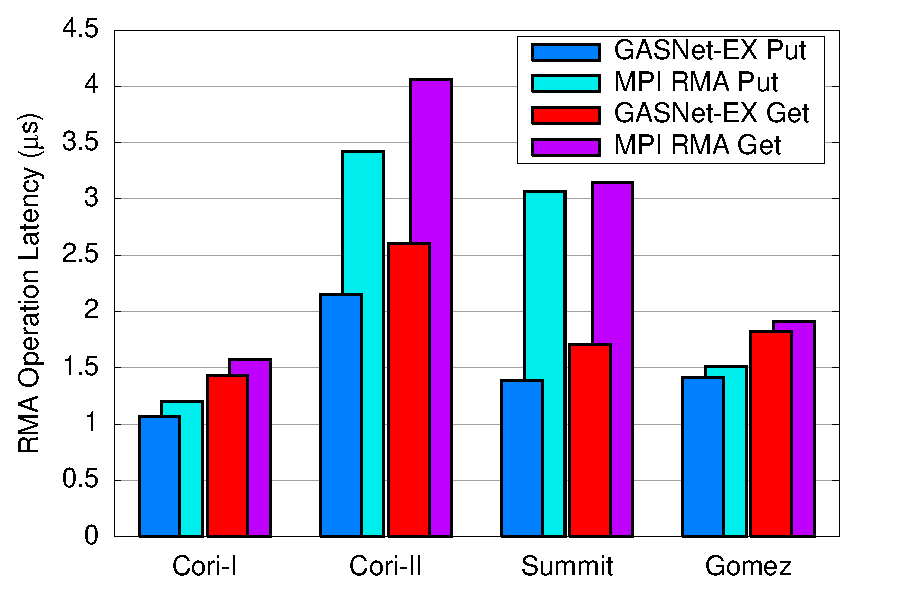
\includegraphics[width=0.432\textwidth]{projects/2.3.1-PMR/2.3.1.14-UPCxx-GASNet/latency_bars.pdf}
  }
  \subfloat[Summit Flood Bandwidth\label{fig:summit-bw}]{
     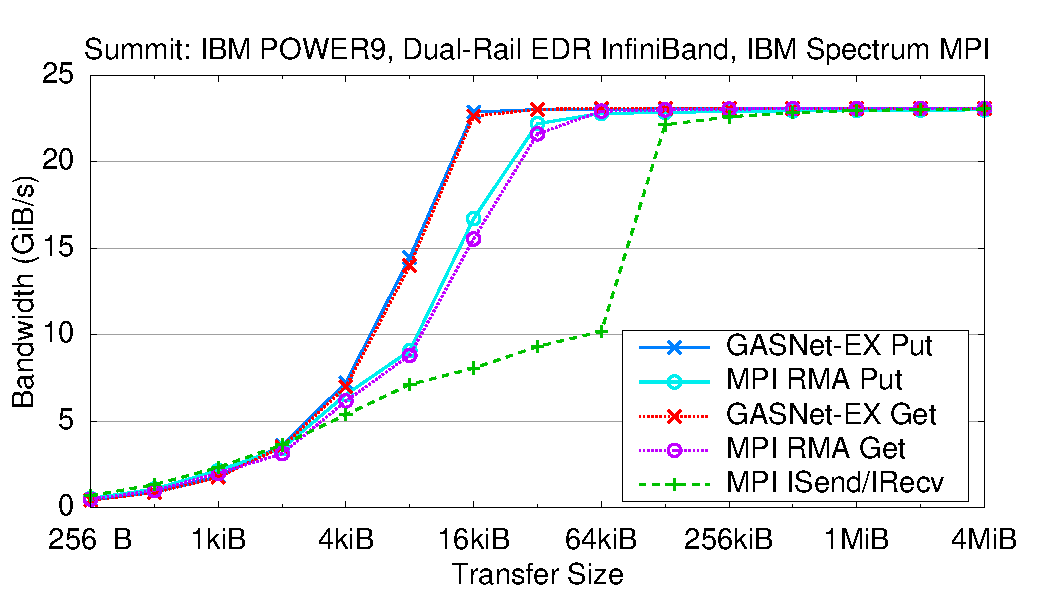
\includegraphics[width=0.504\textwidth]{projects/2.3.1-PMR/2.3.1.14-UPCxx-GASNet/Summit-slide-BW.pdf}
  }
  \caption{\label{fig:gasnet-ex-rma} Selected GASNet-EX vs. MPI RMA Performance Results}
\end{figure}

Figure~\ref{fig:gasnet-ex-rma} shows representative results from a
paper~\cite{gasnet-lcpc18} comparing
the RMA performance of GASNet-EX with MPI on multiple systems including
NERSC's Cori and OLCF's Summit%
\footnote{The paper's results from Summitdev
have been replaced by more recent (June 2019) results from OLCF's newer Summit system.}.
These results demonstrate the ability of a PGAS-centric runtime to
deliver performance as good as MPI, and often better.
%
The paper presents experimental methodology and system descriptions, which are
also available online~\cite{gasnet-site}, along with results for additional
systems.

Figure~\ref{fig:rma-lat-bars} shows the latency of 8-byte RMA Put and Get operations on
four systems, including two distinct networks and three distinct MPI
implementations.
%
GASNet-EX's latency is 6\% to 55\% better than MPI's on Put and 5\% to 45\%
better on Get.
%
Algorithms sensitive to small-transfer latency may become practical in PGAS
programming models due to these improvements relative to MPI.

Figure~\ref{fig:summit-bw} shows flood bandwidth of RMA Put and Get over the
dual-rail InfiniBand network of OLCF's Summit.
GASNet-EX's bandwidth is seen to rise to saturation at smaller
transfer sizes than IBM Spectrum MPI, with the most pronounced differences
appearing between 4KiB and 32KiB.
%
Comparison to the bandwidth of MPI message-passing (dashed green series) illustrates the
benefits of one-sided communication, a major feature of PGAS models.


\paragraph{Recent Progress}

The most notable work on GASNet-EX in the past year has been in two areas:

\textbf{Device (GPU) Memory Support}.
``Memory kinds'' is the GASNet-EX term for support for communication involving
memory other than host memory, and in the context of ECP refers primarily to
accelerator devices such GPUs.
The GASNet-EX APIs for memory kinds have been co-designed with the developers
of UPC++ and the Realm runtime layer of the Legion Programming System
(WBS~2.3.1.08).  In the October 2020 release of a memory kinds prototype for
use by those stakeholders, GASNet-EX can now leverage the GPUDirect RDMA (GDR)
capabilities of modern NVIDA GPUs and Mellanox network adapters (such as those
on Summit) to perform one-sided communication to and from GPU memory without
the overheads of staging through intermediate copies in and out of host memory.

\textbf{Scalability}.
We have devoted effort in the past year to reducing the memory footprint of the
GASNet runtime as the job size grows.  This has included efforts in
collaboration with the ExaBiome (WBS~2.2.4.04) team to run their applications
at previously unattainable scales on Summit at the OCLF and on Cori at NERSC.

\paragraph{Next Steps}

Our next efforts include:

\textbf{Device (GPU) Memory Support}.
We will continue work in the area of GASNet-EX memory kinds, including the
hardening and tuning of the implementation featured in the October 2020
release.  As access to other ECP-relevant systems is secured, we plan to extend
support to accelerators from additional vendors, including those from AMD and
Intel which are scheduled to appear in early Exascale systems.

\textbf{Client-Driven Tuning}.
In collaboration with authors of client runtimes using GASNet-EX (most notably
UPC++ and Legion) and their users (such as ExaBiome), we will continue to
identify and address any significant scalability issues or performance
anomalies which are discovered.

\clearpage
